\subsection{Ziele}

Zu Beginn beschrieben wir den Ablauf einer \ac{HMI} Kommunikation. Dabei sahen die Teilnehmer, dass der Benutzer haptische und akustische Eingaben in das System tätigte und eine visuelle, akustische Ausgabe erhielt. Diese Art der Kommunikation stellten wir als expliziten Kommunikationskanal vor. Dieser zeichnet sich durch die rationalen Informationen aus. Im Gegensatz hierzu stellt der implizite Kanal als Eingabe Emotionen zur Verfügung, worauf der Benutzer eine visuelle, akustische Ausgabe von seinem Kontext empfängt. Schließlich sollte als Eingabe eine haptische und akustische Eingabe der rationalen Informationen dienen, welche mit den Emotionen des Benutzers ergänzt wird, siehe Abbildung ~\ref{fig:communiationskanal}. Hiermit kann eine Anwendung auf die Empfindlichkeiten des Anwenders reagieren. 

\begin{figure}[!h]
	\centering
	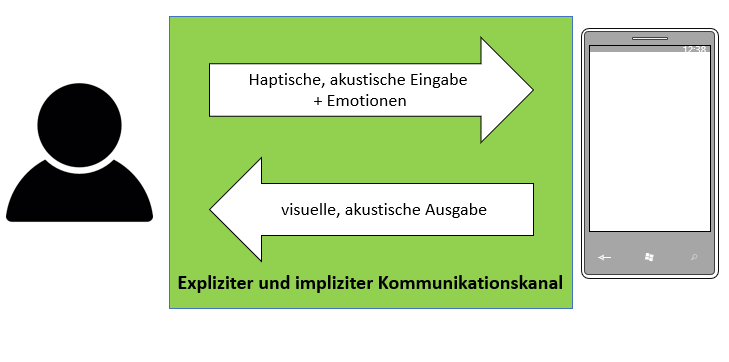
\includegraphics[width=0.9\linewidth]{Pictures/impliziter_expliziter_Kanal}
	\caption[Vereinigung des impliziten und expliziten Kommunikationskanal]{Vereinigung des impliziten und expliziten Kommunikationskanal}
	\label{fig:communiationskanal}
\end{figure}  

Anschließend wurde der Begriff "Affective Computing" eingeführt. Dieser beschreibt ein System, welches Emotionen erkennen, interpretieren und verarbeiten kann. Dabei zeigten wir die von Picard beschrieben Punkte auf, um ein solches System umzusetzen\cite{Picard}:

\vspace{2mm}
\begin{enumerate}
	\item Frustration reduzieren
	\item Klassifizierung der Emotionen
	\item Infrastruktur für Affective Computing schaffen
	\item Emotionale Eigenschaften des Systems trainieren
\end{enumerate}
\vspace{2mm}

Zunächst ist das übergeordnete Ziel die Frustration zu reduzieren. Hierfür können schon einfache Fehlermeldungen reichen, welche die Schuld auf sich nehmen. Für ein intelligenteres System braucht es allerdings noch verschiedene Sensoren, welche Benutzerdaten erfassen. Aus den gesammelten Daten soll nun versucht werden die Benutzeremotionen zu klassifizieren. Sobald das System die Emotionen klassifiziert hat, ist eine Antwort des Systems notwendig. Die Antwort soll natürlich in Zusammenhang mit dem gegebenen Kontext stehen, sodass der Benutzer zielgerichtet angesprochen werden kann.

